\documentclass[12pt]{article}

\usepackage{epsfig}
\usepackage{comment}
\usepackage{natbib}
\usepackage{natbibmnfix}
\usepackage{graphicx}
\usepackage{color}
\usepackage{subfig}
\usepackage{bmpsize}
\usepackage{caption}
\usepackage{amsmath}
\usepackage{breqn}
\usepackage{wrapfig}
\usepackage{lipsum}

\newcounter{dummy}
\def\@biblabel#1{\hspace*{\labelsep}[#1]}

\newcommand{\df}{\delta_{\rm F}}
\newcommand\atf{ATF}

\def\lya{Ly$\alpha$}
\def\lyb{Ly$\beta$}
\def\etal{{\rm et~al.\ }}
\def\hmpc{\;h^{-1}{\rm Mpc}}
\def\hgpc{\;h^{-1}{\rm Gpc}}
\def\hkpc{h^{-1}{\rm kpc}}
\def\kpc{{\rm kpc}}
\def\kms{{\rm \;km\;s^{-1}}}
\def\shear{\langle \gamma^{2} (\theta) \rangle}
\newcommand{\phiv}{\mbox{\boldmath$\phi$}}
\newcommand{\thetav}{\mbox{\boldmath$\theta$}}
\def\pef{\par\noindent\hangindent 15pt}
\def\simlt{\lower.5ex\hbox{$\; \buildrel < \over \sim \;$}}
\def\lesssim{\lower.5ex\hbox{$\; \buildrel < \over \sim \;$}}
\def\simgt{\lower.5ex\hbox{$\; \buildrel > \over \sim \;$}}
\def\apj{{\it Astrophys. J.}}
\def\jcap{{\it  J. Cosmo. \& Astroparticle Phys.}}
\def\aj{{\it Astron. J.}}
\def\mnras{{\it Mon. Not. R. astr. Soc.}}
\newcommand{\apjl}{ApJL}
\newcommand{\nat}{Nature}
\newcommand{\araa}{ARA\&A}
\newcommand{\apjs}{ApJS}
\newcommand{\aap}{A\&A}
\newcommand{\pasp}{PASP}
\newcommand{\sfig}[2]{
\begin{center}
\includegraphics[width=#2]{#1}
\end{center}
        }
\newcommand{\Sjpg}[2]{
    \begin{figure}[htb]
    \sfig{./#1.jpg}{.9\columnwidth}
    \caption{{\small #2}}
    \label{fig:#1}
    \end{figure}
}
\newcommand{\Sfig}[2]{
    \begin{figure}[htb]
    \sfig{./#1.pdf}{.9\columnwidth}
    \caption{{\small #2}}
    \label{fig:#1}
    \end{figure}
}
\newcommand{\Sfigtwo}[3]{
        \begin{figure}[htbp]
\sfig{#1.eps}{.3\columnwidth}
\sfig{#2.eps}{.3\columnwidth}
\caption{{\small #3}}
\label{fig:#1}
\end{figure}
}
\newcommand\be{\begin{equation}}
\newcommand{\Rf}[1]{\ref{fig:#1}}
\newcommand{\rf}[1]{\ref{fig:#1}}
\def\ee{\end{equation}}
\def\bea{\begin{eqnarray}}
\def\eea{\end{eqnarray}}
\newcommand{\vs}{\nonumber\\}
\newcommand{\ec}[1]{Eq.~(\ref{eq:#1})}
\newcommand{\Ec}[1]{(\ref{eq:#1})}
\newcommand{\eql}[1]{\label{eq:#1}}
\newcommand\cov{{\rm Cov}}
\newcommand\cl{{\mathcal{C}_l}}
\usepackage[margin=3.0cm]{geometry}
\usepackage{pslatex}
\newcommand\fnl{f_{\rm NL}}
\newcommand{\wh}[1]{\textcolor{blue}{[#1]}}

\newcommand\cp{C^{pri}}
\newcommand\ci{C^{ISW}}
\newcommand\cg{C^{gg}}
\newcommand\cgt{C^{g-ISW}}
\newcommand\tob{T^{\rm obs}}
\newcommand\aob{a^{\rm obs}}
\newcommand\tisw{T^{\rm ISW}}
\newcommand\aisw{a^{\rm ISW}}
\newcommand\si{C^{\rm ISW}_l}
\newcommand\sig[1]{C^{\rm g_{#1}-ISW}_l}
\newcommand\sg[2]{C^{\rm g_{#1}g_{#2}}_l}
\newcommand\tp{T^p}


%
% definitions
%
% A useful Journal macro
\def\Journal#1#2#3#4{{#1} {\bf #2}, #3 (#4)}
% Some useful journal names
\def\NCA{\em Nuovo Cimento\ }
\def\NPB{{\em Nucl. Phys.} B\ }
\def\PLB{{\em Phys. Lett.}  B\ }
\def\PRL{{\em Phys. Rev. Lett.\ }}
\def\PRD{{\em Phys. Rev.} D\ }
\def\prd{{\em Phys. Rev.} D\ }
\def\ZPC{{\em Z. Phys.} C\ }
\def\apj{{\em Ap. J.\ }}
\def\apjl{{\em Ap. J. Lett.\ }}
\def\la{\hbox{${_{\displaystyle<}\atop^{\displaystyle\sim}}$}}
\def\ga{\hbox{${_{\displaystyle>}\atop^{\displaystyle\sim}}$}}



\baselineskip=11pt
\def\msun{{\rm M_{\odot}}}

\textheight=24.3cm
\textwidth=16.8cm

\begin{document}
\topmargin=-2.105cm
\oddsidemargin=-0.1cm
\evensidemargin=0cm

\begin{center}
%{\LARGE \bf Weak lensing from anisotropies in the two point correlation function: precision cosmology from new tracers}
{\LARGE \bf New Vistas in Weak Lensing}
\end{center}

\begin{small}



\section{Overview and Objectives}
Weak gravitational lensing 
has emerged as one of the powerful probes of the
structure of the Universe and ways of distinguishing cosmological models. The 
small distortions of background images as they are lensed by foreground matter
are sensitive to both the matter contents and the geometry of the Universe
(e.g., \cite{blandford92}, \cite{hoekstra2008}).
Galaxy images are the most commonly used cosmological 
sources (see \cite{Kilbinger2015} and references therein),
but weak lensing of the cosmic microwave background (CMB) 
is also widely studied (see e.g., the review by \cite{lewis2006}, and results from, e.g., the Planck satellite, Ade {\it et
 al.} 2015). 
 
These two very successful implementations of lensing are similar in that they both are sensitive to -- and therefore can be used to measure -- the projected gravitational potential as a function of position on the sky:% {\bf this needs to be fixed}:
\begin{equation}
\Phi(\vec\theta)=\frac{2}{c^2}\int^{D(z_{s})}_{0}\frac{dD}{D(z_s)}\,\frac{D(z_{s},z)}{D}\phi(\vec x),\eql{phi}
\end{equation}
where $\phi$ is the 3D potential at the position $\vec x=\vec x[\vec\theta,D(z)]\rightarrow [D(z)\vec\theta,D(z)]$ in the small angle limit; $D(z)$ is the angular diameter distance to redshift $z$ and $D(z,z')$ is the angular diameter distance between redshifts $z$ and $z'$. However, they
differ not only in the sources that are studied (galaxies in one case and the CMB in the other) but also in the fundamental observable that is used to extract information about $\Phi$: in one case, the distorted shapes of the galaxies are used to infer information about the intervening mass, while in the case of the CMB, the inhomogeneous potential leads to {\it anisotropies} in the two-point statistics of the otherwise Gaussian field. 

\newcommand\atf{ATF}
Since so much of this proposal will be based on the anisotropy in the 2-point statistics and because this idea is relatively new \citep{Hu:2001tn} compared with the easier to understand shape measurements, it is worth spending a paragraph outlining the basic idea. Since the universe is homogeneous and anisotropic, the two-point function of any observable, e.g., the temperature on the surface of last scattering: $C(\phi)=\langle T(\vec \theta)T(\vec\theta+\vec{\phi})\rangle$ depends only on the magnitude of $\vec\phi$. When expanded in terms of spherical harmonics with coefficients $a_{lm}$, this property leads directly to the relation
\be
\langle a_{lm} a^*_{l'm'}\rangle = \delta_{ll'}\delta_{mm'} C_l
.\ee
When photons from one part of the sky travel through an over-dense region and from another through an under-dense region, the situation changes and now the 2-point function depends not only on angular distance between two points but also on the position on the sky. The product of $a_{lm}$ and $a_{l'm'}$ now will have non-zero expectation even when $l\ne l'$, an expectation value that is proportional to the field that breaks the isotropy, $\Phi$. By forming quadratic estimators with $lm$ and $l'm'$ slightly different, we can obtain an estimate for the potential~\citep{Hu:2001tn,okamoto}. For simplicity, we will refer to this effect as {\it anisotropic two-point functions}, or simply \atf.
 
\atf\ of the CMB field has proved fruitful, but it is not the only possibility, as any light emitted
at cosmological distances is deflected on its way to us and therefore the statistics of any set of sources will be anisotropic. With the huge
growth in surveys of the Universe we now have the exciting possibility
of expanding the way gravitational lensing is done and treating new
fields and new observations as sources. In the context of this more general
view of weak lensing, we have chosen two of the most
promising sources to focus on, the Lyman-alpha forest, and 
angular galaxy clustering. Fig.~\rf{table} gives a schematic view of the new vistas that can open up when we move beyond the CMB as a source.

\Sfig{table}{Schematic overview of this proposal: shapes of source galaxies (upper left) and quadratic estimators that exploit the impact of lensing on the CMB two-point functions (middle panel) have matured in recent years so that they are used to estimate cluster masses (left figure in each panel) and make maps of the large scale structure of the universe (right figure in each panel). This proposal aims to expand the tool of lensing on two-point functions to the cases where galaxies (left, middle) and the Lyman alpha forest (right, middle) are the sources. Finally, it aims to use some of the same techniques to detect time delays from photons in the CMB (bottom row). In principle, time delays can also impact the two-point functions of galaxies (left, bottom) and the Lyman alpha forest (right, bottom), but we think the current focus of the proposal on the three shaded boxes presents a broad range of opportunities for students: ranging from guaranteed detections that could become competitive to more speculative ideas that will likely yield detections, but more work is needed to demonstrate that they can provide information competitive with the more traditional lensing methods.}

For the first probe, the \lya\ forest, we note that as the angular 
positions of quasars are deflected by the 
gravitational lensing effect of foreground matter, the \lya\ forest 
seen in the spectra of these quasars is 
therefore also lensed.
In \cite{croft17} (hereafter C18)
 the PI proposed that the 
\atf\ of the \lya\ forest
can also be measured.
%(e.g., \cite{zahn2006}). 
%As with 21cm data, 
The forest has the advantage of spectral information,
potentially yielding many lensed ``slices'' at different redshifts.
An idealized test was carried out in C18 using
using a mock  high resolution angular grid of quasars (of order arcminute separation) and a linear theory foreground density
field. Standard quadratic estimators (e.g., \cite{okamoto})  
were used to successfully  reconstruct images of the foreground mass 
distribution. In the work proposed here we will expand the realism
of such tests and make measurements on real data. Enough work has been done to date on this source that this is a relatively low risk
project. There is still the question of how powerful a tool \atf\ of the \lya\ forest statistics will become. Will they surpass the more traditional shape measurements for at least some range of redshift? What are the systematics that must be treated in order to extract cosmological information. We argue below that we are well-suited to address these questions and feel that they provide a broad range of opportunities for graduate students.

Our second new probe, the \atf\ 
of the angular galaxy distribution,
relies on the same physics. The positions
of galaxies are deflected by the gravitational potential produced by
foreground matter. This manifests itself in local distortions of
clustering statistics of qualitatively 
the same type which are measured in CMB lensing.
In the past, the number density of galaxies in large-area surveys 
was not sufficient to overcome the shot noise inherent in deriving
the lensing potential from the discrete galaxy distribution. This is
no longer the case however (as we show below, in this proposal), and
this offers a route to galaxy-based lensing constraints without
galaxy shape measurement.

Finally, as indicated in Fig.~\rf{table}, we propose to use \atf\ to open up a new window on time delays. Until now, these have been detected only in the case of strong lensing. But using the new technique, we show that upcoming CMB experiments can estimate the time delay field on the largest of scales. The projected potential responsible for time delays differs from that in \ec{phi} in that it does not contain the second ratio of distances in the integrand and therefore its measurement probes the potential along a given line of sight with a different weighting factor in redshift. Besides this feature, the possibility of measuring properties of the universe on the largest scales possible opens up windows on understanding anomalies that have been observed at the 2-3 sigma level on large scales. 

We will carry out an in depth study of 
the weak lensing of these three new probes, spanning theory, 
simulations and first detections. 
We will study them together over the proposed period in order to benefit from
their common aspects (e.g., the role of angular deflections), common
simulations and
the differing experience and perspectives of the PI and Co-PI.
Mock catalogs and  real 
data will be used
 to understand what can be achieved and to gain physical understanding
from it. Our ultimate aim is to develop these lensing tracers as new tools
for cosmology, and to motivate 
observing strategies.
Our specific objectives are as follows:

(a) {\bf \underline{to simulate new lensing tracers,}} the Ly$\alpha$ forest and galaxy clustering,
 including non-linear physics, baryonic effects and observational
systematic errors.

(a) {\bf \underline{to develop statistical techniques}} for the analysis of new lensing data, including 
cross-correlations and mass reconstruction, and use knowledge from our full simulations to address and mitigate systematics.


(c) {\bf \underline{to make observational measurements}} spanning first 
detections to precision measurements of $\sigma_{8}$ at the 3\% level 
from different datasets, the CLAMATO, eBOSS and DES surveys.

(d) {\bf \underline{to explore new cosmological constraints}} from these
measurements which have different strengths and potential biases  to other
lensing results.


\input{intro.tex}
\subsection{\lya\ forest lensing}


An idealized test was carried out in C18 using using a mock high
resolution angular grid of quasars (of order arcminute separ\ ation)
and a linear theory foreground density field. Standard quadratic
estimators (e.g., \cite{okamoto}) were used to successfully
reconstruct images of the foreground mass distribution. In the work
proposed here we will expand the realism of such tests and make
measurements on real data. Enough work has been done to \ date on this
source that this is a relatively low risk project. There is still the
question of how powerful a tool \atf\ of the \lya\ \ forest statistics
will become. Will they surpass the more traditional shape
mea\ surements for at least some range of redshift? What are the
systematics that mu\ st be treated in order to extract cosmological
information. We argue below that\ we are well-suited to address these
questions and feel that they provide a bro\ ad range of opportunities
for graduate students.




The \lya\ forest of absorption features due to neutral hydrogen can
seen in the spectra of both quasars \cite{rauch1998} and galaxies (e.g.,
\cite{savaglio2002}).  We refer to quasars and galaxies as
``backlights'' rather than ``sources'' in what follows, in order to
avoid confusion with the ``sources'' in gravitational lensing (which
will be the \lya\ forest here). At the redshifts ($2 < z
< 6$) where the \lya\ transition is in the optical wavelength
range, the forest absorption mostly arises in the moderately overdense
(of order the cosmic mean) intergalactic medium (IGM) (\cite{bi1993}, 
\cite{cen1994}, \cite{zhang1995}, \cite{hernquist1996}).
  This intergalactic medium is a continuous field, and as such
\lya\ forest spectra can be thought of as a collection of
one-dimensional ``intensity maps'',
where the relevant property is the ``flux overdensity'', $\df=\frac{F}{\langle F \rangle} -1$ ($F$
is the transmitted flux in a spectrum).  Its properties are well
studied and it is relatively easy to simulate numerically (see e.g.,
\cite{bolton2017}). The forest has been used to test
cosmological models, for example through the influence of the neutrino
mass on large-scale structure (e.g., \cite{pal2015}, \cite{croft1999}).
  With a high enough angular
density of quasars, three dimensional statistics can be evaluated by
using information from multiple sightlines, enabling clustering
measurements and detection of baryon
oscillations \citep{busca2013},. The
collection of one-dimensional skewers can also be used to make
continuous three dimensional maps using a variety of interpolation
techniques (e.g., \cite{cisewski}), and
with even more numerous star forming galaxies as background spectra
these can be made with angular resolution close to arcminute scales
\citep{Lee2014}.

The \lya\ forest, being measured from spectra has a precisely known
source redshift. This fact is also advantageous for lensing of the
CMB, enabling analyses to be free of uncertainties in the redshift
distribution of sources which affect galaxy weak lensing studies
\citep{hearin2010}.


The \lya\ forest at redshift $z_{s}$ is lensed by the matter
distribution lying between us and $z_{s}$. Gravitational lensing
shifts the observed positions of points on the sky without changing
their surface brightness.  In the case of the \lya\ forest, this means
that the quasar or galaxy backlights move on the plane of the sky.
The angular sizes of quasars are magnified (through the change in
their angular sizes). This magnification of quasars through lensing is
well studied, from the first observed lenses, which created multiple
quasar images \citep{walsh1979}, through weak lensing
magnification of quasars detected by cross-correlation with foreground
galaxies (e.g., \cite{scranton2005}).  The magnification of
quasars will cause some selection biases which we plan to investigate
with mocks. Directly relevant to \lya\ forest lensing, however
are distortions of the angular separations between quasars, caused by
the lensing deflection of light. 
  Gravitational lensing therefore distorts the ``image'' of the 
IGM probed by the \lya\ forest without
changing the transmitted flux measured in each pixel. This is directly
analogous to the effect of lensing on 21cm emission (or the CMB),
which conserves surface brightness.  In
the left panel of Figure \ref{cartoon} we
illustrate this with a diagram, which shows the \lya\ forest pixels
being deflected in a similar fashion to the quasar backlights. In
the right panel of 
Figure \ref{cartoon} we concentrate on a single backlight and \lya\
forest pixel and show the relationship to the unlensed angular
positions of both. The pixel and the backlight are at different
angular size distances, and so are displaced on the sky by different
angles.

\begin{figure}
  \begin{center}
    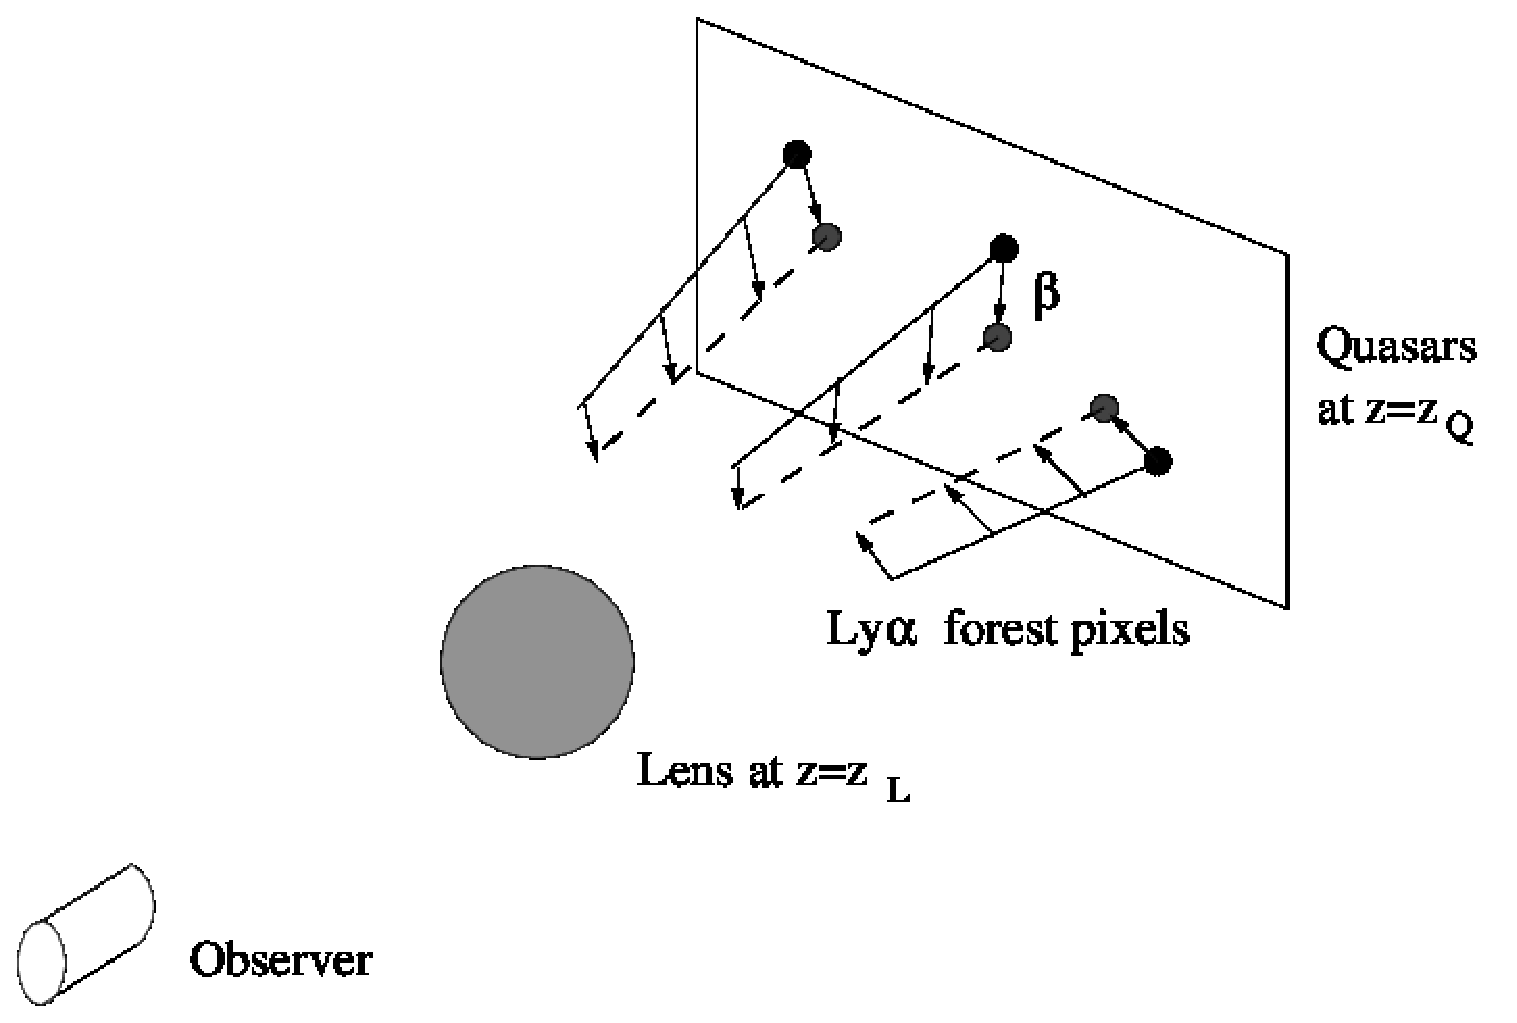
\includegraphics[scale=0.33]{figs/lensdiagram.eps}
    \hspace{1cm}
    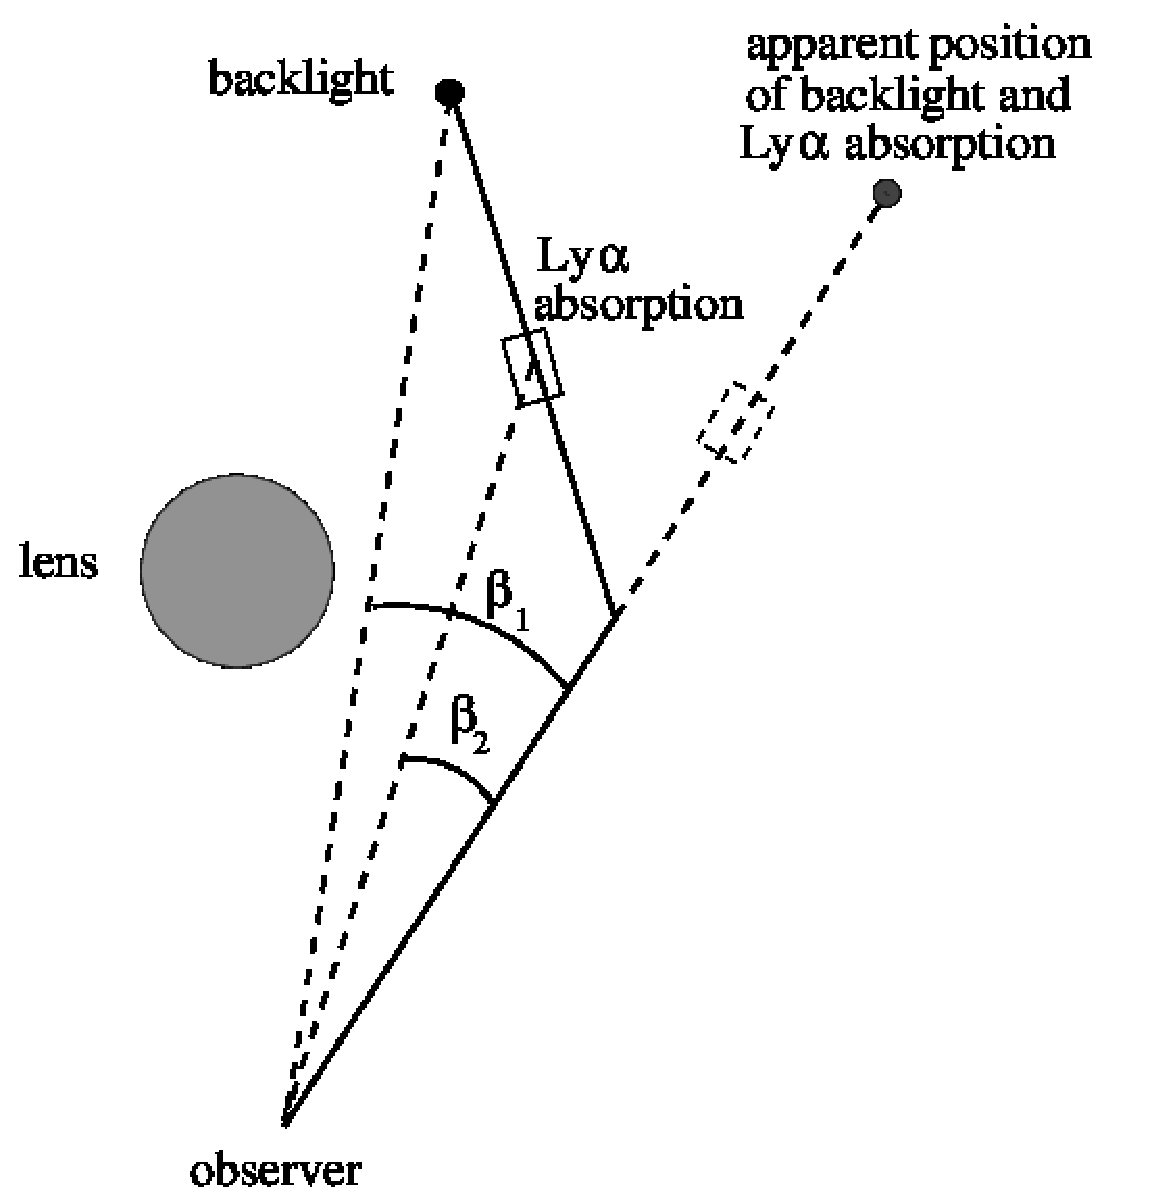
\includegraphics[scale=0.33]{figs/angdiag.eps}
  \end{center}
  \caption{
{\bf Left panel: cartoon illustration of the geometry of \lya\ forest lensing.}
Due to lensing by the foreground object at redshift $z_{L}$, the 
angular position of a quasar at redshift $z=z_{Q}$ is 
deflected by an angle $\beta$. The associated
\lya\ forest pixels are also lensed, deflected by an angle smaller than 
$\beta$ 
(which depends on the angular size distance to the absorption in the pixel).
{\bf Right panel: lensing deflection for a single \lya\ forest pixel.}
The deflection angle for the backlight ($\beta_{1}$) is different 
from that for the \lya\ forest absorption    ($\beta_{2}$) because they are 
at different redshifts (and                       therefore angular size distances).
           }
  \label{cartoon}
\end{figure}


If the lensing deflections are small
compared to structure in the source, the \lya\ forest 
flux overdensity $\df$  at wavelength $\lambda$ can
be expressed as a Taylor expansion of the unlensed $\df$.

\begin{equation}
\widetilde{\delta}_{F}({ \pmb {\theta}},\lambda)=
{\delta_{F}}({ \pmb {\theta}} - {\pmb { \alpha}}({\pmb {\theta}}) ,\lambda)
\simeq {\delta_{F}} ({\pmb{\theta}},\lambda) - {\pmb {\alpha}}({\pmb{\theta}})\c
dot
{\pmb{\nabla_{\theta}}} \delta_{F} ({\pmb{\theta}},\lambda) + ...
%\delta_{F}({\bf \theta-\alpha(\theta)}, \lambda) 
%\simeq \delta_{F}({\bf \theta},\lambda)
\label{taylor}
\end{equation}

 This expansion is  valid in the case of the \lya\ forest, where gradients
in $\delta_{F}$ can be large, but the deflections (or deflection gradients) 
are small compared to them on all scales of interest. The deflection field
${\pmb {\beta}}( {\pmb {\theta}})$ is related to the 2D projected lensing potent
ial via
${\pmb {\nabla \Phi}} =- {\pmb {\beta}}({\pmb {\theta}} )$,
in the weak lensing limit. This lensing potential can be
computed from the full 3D gravitational
potential (e.g, Bartelmann \& Schneider 2001) by an integration
over redshift as in \ec{phi}.
This lensing potential
can  be reconstructed from the \lya\ forest field using 
quadratic estimators (e.g., \cite{okamoto}).


\subsection{Galaxy Clustering}\label{sec:lia}

%\subsubsection{Motivation}

\subsubsection{The Effect}
The simplest statistic that
characterizes the angular distribution of galaxies on the sky is the
angular correlation function, $w(\vec\theta_1,\vec\theta_2)$, which
quantifies the excess probability over random that a galaxy will be
found at $\vec\theta_2$ given that there is a galaxy at
$\vec\theta_1$. In the isotropic case, the angular correlation function depends only on the angular distance
between the two positions: $w=w(\vert\vec\theta_1-\vec\theta_2\vert)$. The \atf\ effect here means
that $w$ depends also on the location on the sky.

%\begin{figure}
%  \begin{center}
%    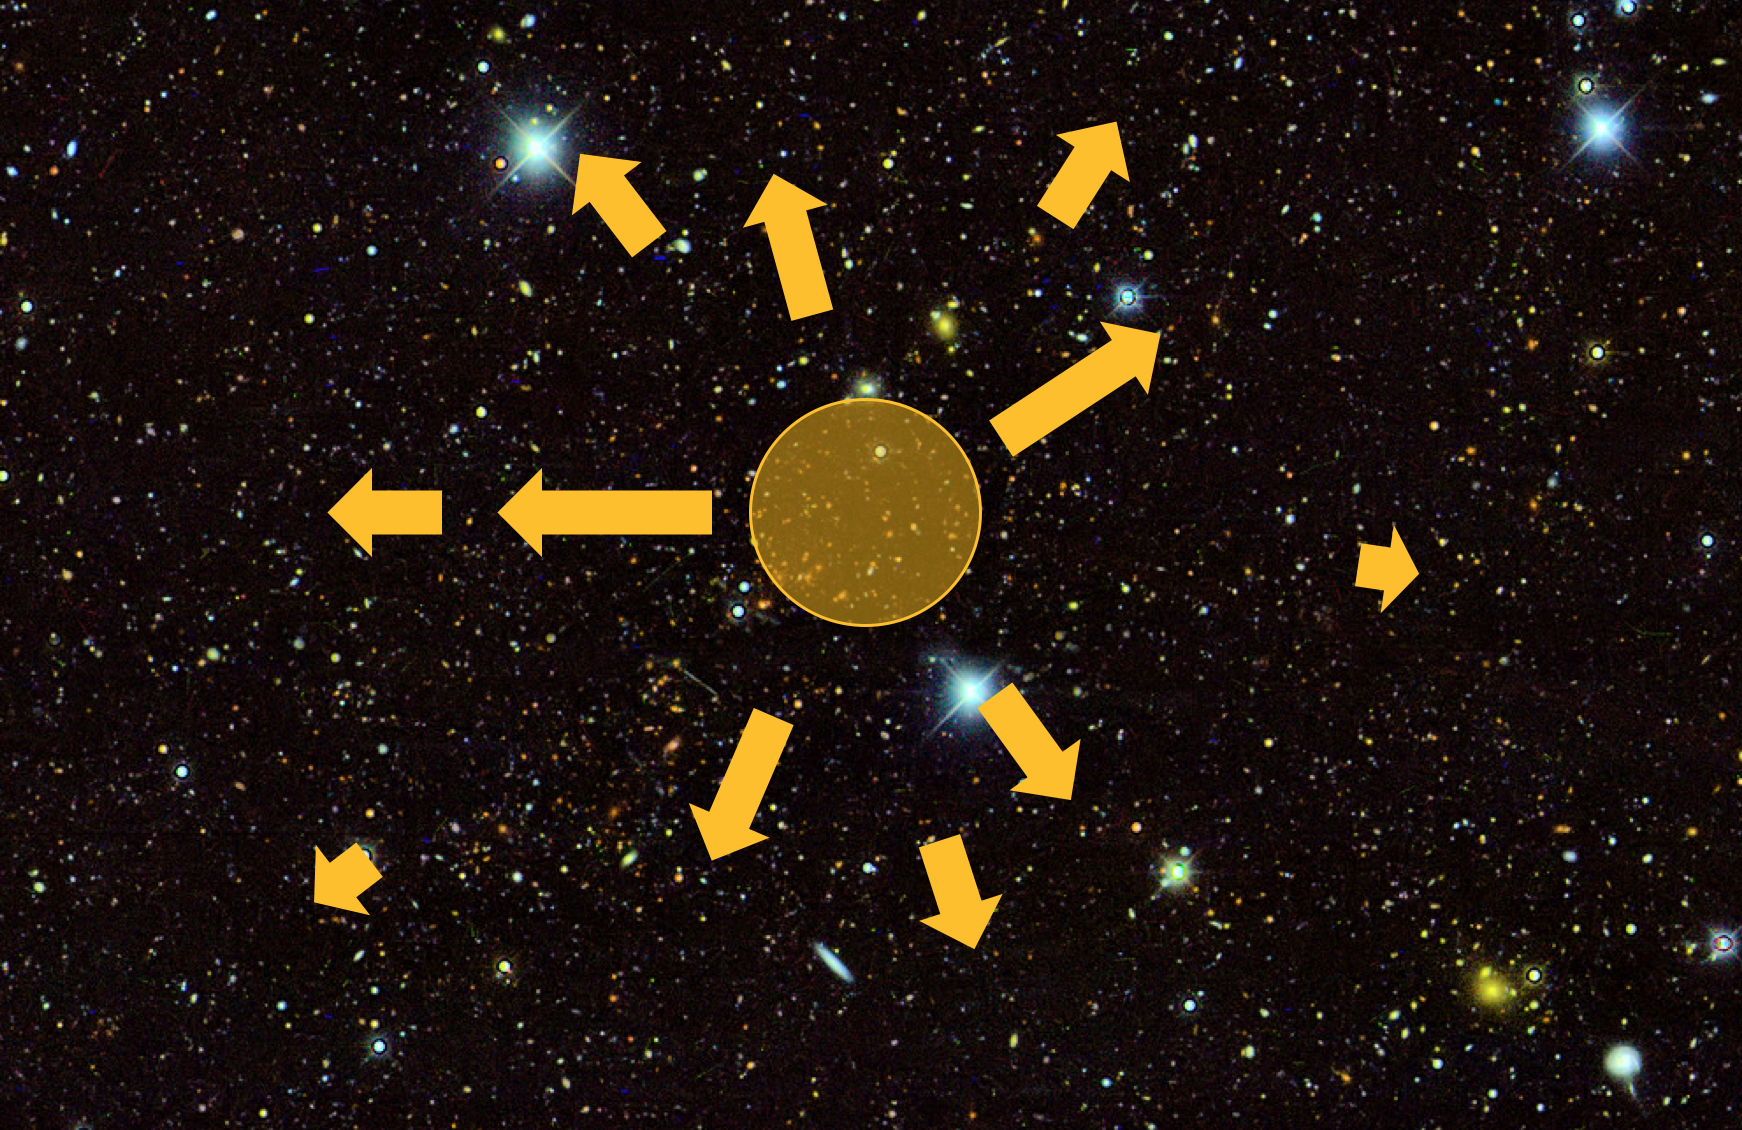
\includegraphics[scale=0.2]{figs/clusterfig.jpg}
%  \end{center}
\begin{wrapfigure}{R}{0.4\textwidth}
\centering
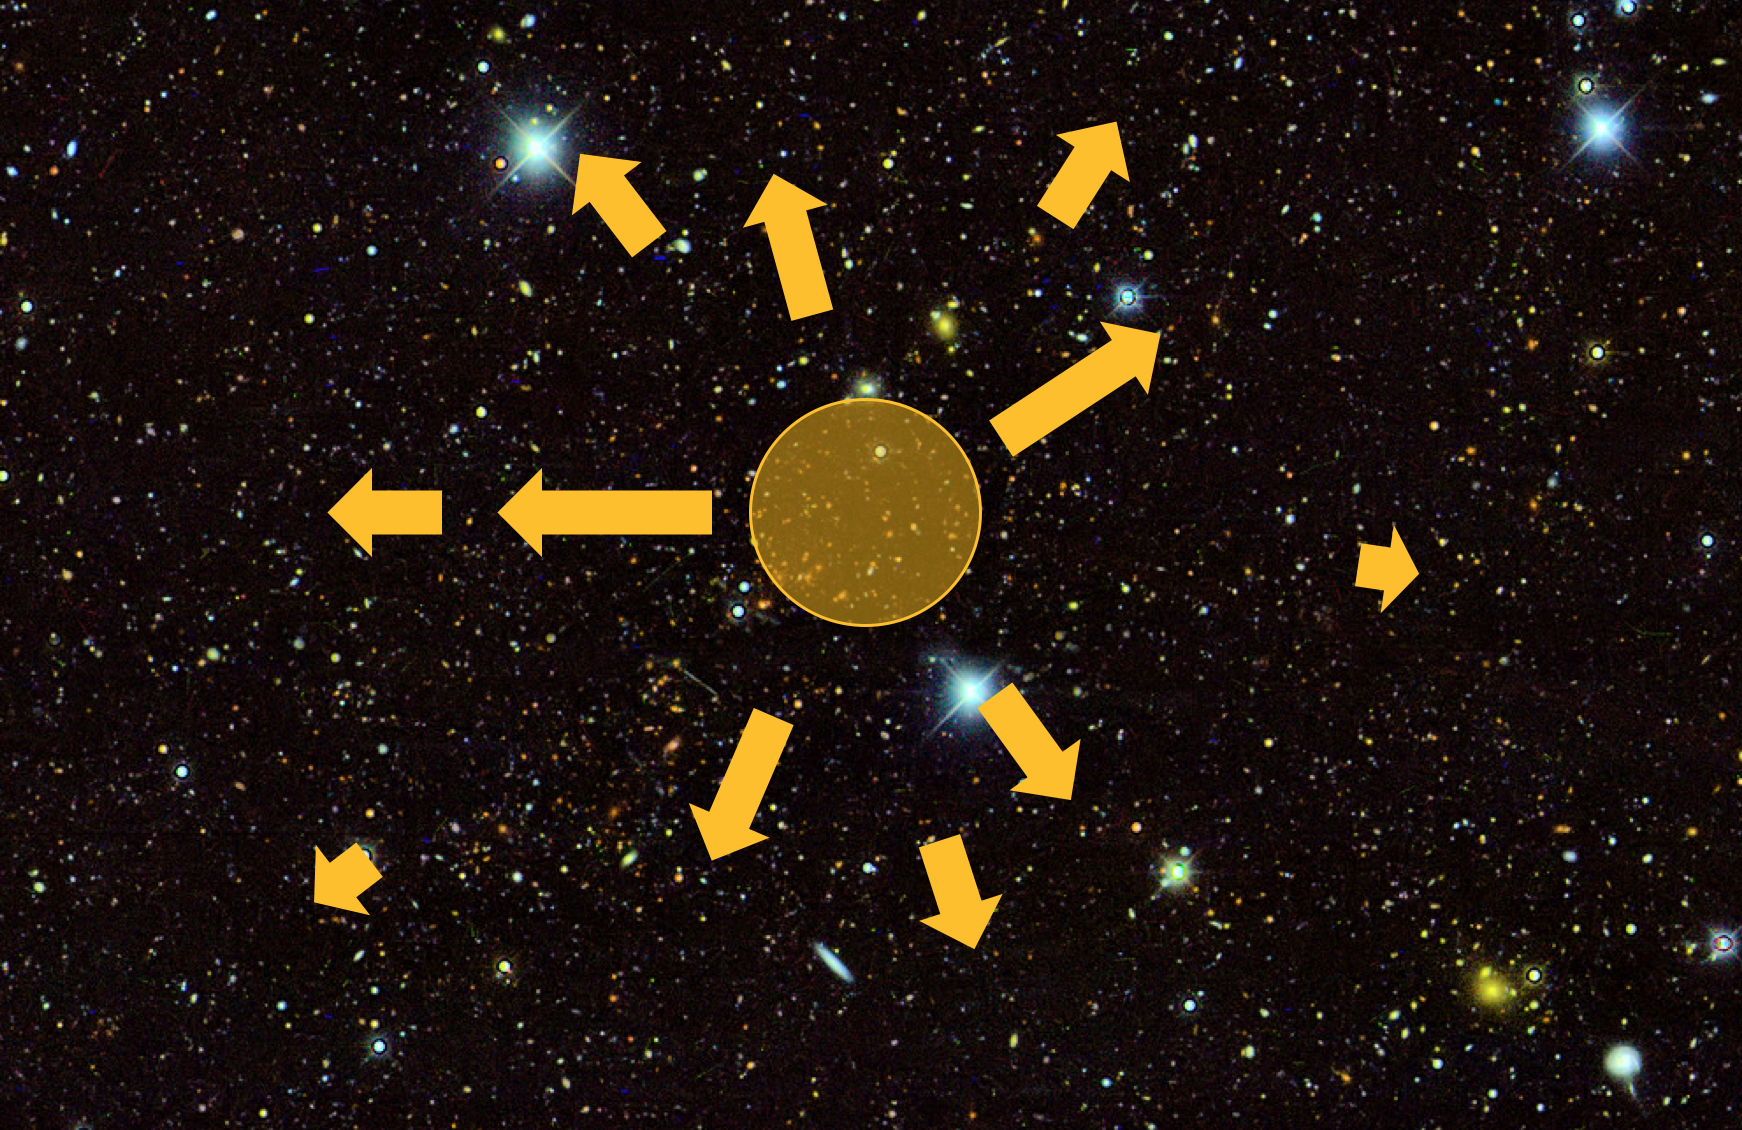
\includegraphics[width=0.4\textwidth]{figs/clusterfig.jpg}
  \caption{ \footnotesize
{\bf Cartoon of the impact of a foreground lens on
  background galaxies.} All galaxies appear further away from the
  cluster center, their observed positions shifting as
  indicated by the arrows. Galaxies closest to the center experience
  the largest shift in position (this 
lensing deflection is not shown to scale). The correlation function
of the background galaxies will also be distorted by these deflection
angles, and this is what we plan to measure.}
  \label{cluster}
\end{wrapfigure}
%\end{figure}

This is simplest to envision and to measure when measuring $w$ behind a massive object such as a galaxy cluster. 
Fig.~\ref{cluster} shows a schematic picture of this. For example, the positions of the two galaxies directly to the left of the cluster are deflected by different amounts (the one closest is deflected more than the one further away, so the observed distance between those two galaxies is {\it smaller} than it would be in the absence of lensing. The observed $w$ then is governed by the larger unlensed distance. Walking through this exercise for all pairs of galaxies in the picture make it clear that the observed $w$ will not depend on simply the observed angular distance between pairs of galaxies. Indeed, we argue that {\bf the 
most impactful implementation of the \atf\ of galaxies will be to measure the masses of galaxy clusters.}


%
%
%This assumption breaks down in the real universe where different lines
%of sight pass through over- or under-dense regions. The observed
%angular correlation therefore depends on the angular positions of the
%two galaxies: $w=w(\vec\theta_1 ,\vec\theta_2)\ne
%w(\vert\vec\theta_1-\vec\theta_2\vert)$. We propose to use this {\it
%  anisotropy of the correlation function} to learn about the structure
%between us and the background galaxies. We will first detect this
%behind the most massive objects, galaxy clusters, and then move to
%measure the anisotropy on the full sky, where it is induced by the
%various under- and over-dense regions that constitute the cosmic
%web. To be clear, the variety of non-gaussian effects that impact the
%distribution of galaxies on the sky do {\it not} break isotropy so
%cannot be confused with this effect.

\subsubsection{Context}

Galaxy clusters are the largest, most massive bound structures in the
universe and therefore are the key to a number of cosmological
puzzles. Chief among these is identifying the mechanism responsible
for the current epoch of cosmic acceleration. The community has moved
on from simply measuring the equation of state of a hypothetical dark
energy substance. There is now a concerted effort to test the
canonical $ \Lambda$CDM predictions both for the expansion history of
the universe and for the rate of the growth of structure. Galaxy
clusters offer the potential for testing both of these predictions:
the number of rare objects such as clusters at a given time is
exponentially sensitive to the RMS fluctuations in the density field,
so cluster abundance at multiple redshifts can be translated into measurements of the growth function. Similarly, the abundance is
sensitive to the volume of a given redshift slice, which depends on
the redshift-distance relation.

The one impediment to date of using clusters as a powerful tool is the
uncertainty in cluster masses. However, we are entering an exciting
epoch that promises to change this situation. Besides the large
surveys now online and coming online in the 2020's, five ways of
inferring cluster masses have emerged and using all of them together
leads to the hope that the systematic uncertainties in any one of them
will not induce a large bias. The techniques of interest are: cluster
richness, X-Ray luminosity, Sunyaev-Zel'dovich signal induced by hot
electrons in the intracluster gas, weak lensing by galaxies, and most
recently weak lensing by the cosmic microwave background 
(CMB)~\cite{Liu:2014pqa,Baxter:2014frs,2014MNRAS.439.1628Z,melchior2017,simet2017,Baxter:2017ixz}. This
proposal aims to add yet another tool that can measure galaxy cluster
masses. Dodelson has not only helped launch the field of CMB cluster lensing with \cite{Baxter:2014frs}, but also serves as Co-Chair of the
Dark Energy Survey Science Committee. He brings insight into the DES cluster cosmology analysis. The Year 1 analysis will be released by the time this proposal is read, and we are currently working on Year 3 data. From the estimates below, it is possible that \atf\ of galaxies will emerge as a powerful tool for cluster cosmology even for DES data. The situation is even more promising for next generation surveys, such as LSST.



%Of course, using the anisotropy in clustering
%statistics has been exploited already in studies of the cosmic
%microwave background.  The small scale structure of the CMB carries
%information about the lensing potential along the line of sight. This
%information has now been extracted by multiple CMB experiments,
%obtaining maps of the integrated gravitational potential and
%information about the masses of clusters. There are differences
%between the lensing-induced anisotropies proposed here and those
%produced by lensing of the CMB. First, the information in the CMB is
%currently limited by the resolution of the telescopes to be about
%$1'$, while galaxy surveys that measure galaxies do much better,
%resolving galaxies separated by several arcseconds. Second, the
%primary CMB is predominantly a Gaussian field, while the small scale
%galaxy distribution has evolved to be very non-gaussian\footnote{A
%  technical point: the impact of lensing produces an anisotropic field
%  in both the cases of the CMB and galaxy clustering. In the former
%  case, the anisotropic field is Gaussian, while in the latter it is
%  non-gaussian. In both cases, though, the effect is characterized by
%  $w\ne w(\vert\vec\theta_1-\vec\theta_2\vert)$.  The distinction between the Gaussian (CMB) and non-Gaussian (galaxies) manifestations
%  of lensing disappears when one considers the power spectra of the
%  lensing field: these are estimated via a 4-point function, which is
%  non-gaussian in both cases.}.
%
%The difference in scales suggests that the route into this new effect
%of the clustering anisotropy induced by lensing is by first detecting
%it when the lenses are discrete objects such as clusters. Upcoming
%surveys will find hundreds of galaxies -- and therefore tens of
%thousands of pairs of galaxies -- in the few square arcminute field
%behind a galaxy cluster. As we show below, this leads to an exciting
%opportunity to open up this new area of lensing. The fact that the
%signal scales with the number of pairs of galaxies and the fact that
%the shapes of these galaxies do not need to be measured reflect two
%advantages over the current weak lensing estimates of cluster
%masses. After detecting this effect behind clusters, we will turn to
%large scale mapping of the integrated gravitational potential. Here,
%the problem becomes similar to the CMB because the galaxy field on
%large scales is close to gaussian, so many of the tools developed in
%CMB lensing can be imported. Indeed, cross-correlating the maps
%produced by the CMB and those produced by galaxy fields will be a
%powerful way to reduce the systematic effects that afflict each
%separately.
%



\subsubsection{Signal to Noise}

Let us provide a rough estimate of the detectability of
the \atf\ of the galaxy distribution due to a typical cluster of mass $2\times10^{14} M_\odot$. We can assume that the
unlensed $w(\theta)$ is known extremely well because it can be measured over the large area covered by any modern survey (e.g., in DES, this is 5000 square degrees and 20,000 in LSST). The observed
correlation function of the background galaxies will be distorted due to the presence of the
foreground lens, as in the cartoon in Fig.~\ref{cluster}. Each
galaxy's position will be shifted: \be \vec\theta^{\rm obs} =
\vec\theta + \vec{\delta\theta}(\vec\theta) \ee where $\vec\theta$ is
the undeflected position, and the deflection angle $\vec
{\delta\theta}$ is a function of $\vec\theta$ that depends on the mass
distribution of the lens. For the purpose of this estimate, we assume a point mass
lens, \be \vec{\delta\theta}(\vec\theta) =
\vec\theta\,\frac{\theta_E^2}{\theta^2}. \ee For a lens a typical distance of 1 Gpc from us (and sources far behind),
the Einstein radius $\theta_E=40'' (M/2\times 10^{14}M_\odot)^{1/2}.$ 





The unlensed positions are $\vec\theta^{\rm obs}-\vec{\delta\theta}$,
and the correlation function governing those unlensed positions is
$w(\theta)$. Therefore, the observed angular correlation function
between two positions $\vec\theta_ i$ and $\vec\theta_j$ is \be w^{\rm
  obs}(\vec\theta_i^{\rm obs},\vec\theta_j^{\rm obs}) = w(\vert
\vec\theta _i^{\rm obs} - \vec{\delta\theta}(\vec\theta_i) -
\vec\theta_j^{\rm obs} + \vec {\delta\theta}(\vec\theta_j)\vert).  \ee
For the purposes of estimating the magnitude of this effect, we now
make the approximation that the deflections are small, so the
argument of $w$ on the right -hand side can be Taylor expanded. Note
that this approximation is not essential, as in the case of CMB
cluster lensing~\cite{Baxter:2014frs} we avoided it by using a likelihood approach, but
this will be the first step in our program. Taylor expanding and dropping the $^{\rm obs}$ superscript on the angles leads to \bea
w^{\rm obs}(\vec\theta_i,\vec\theta_j) &=& w(\theta_{ij}) +
w'(\theta_{ij})\left[ \vec{\delta\theta}(\vec\theta_i) -
\vec{\delta\theta}(\vec\theta_j) \right]\cdot
\frac{\vec\theta_i-\vec\theta_j}{\vert
  \vec\theta_i-\vec\theta_j\vert}\vs &\equiv &w(\theta_{ij}) +
w'(\theta_{ij}) f_{ij} \eql{taylor} \eea where here $\theta_{ij}\equiv
\vert\vec\theta_i-\vec\theta_j\vert$; $w'\equiv d w/d\theta$, which
can be measured extremely accurately from all other patches in the
survey; and the second line condenses the additional terms to save
space.


The second term in \ec{taylor} is the effect we are after, the signal,
as it contains the information about the deflection angles that
depend on the mass of the lens. To estimate the signal to noise, we
imagine pixelizing the region around the lens and forming an
estimator for the angular correlation function for every pixel pair:
\be \hat w(\vec\theta_i,\vec\theta_j) = \delta_i\delta_j \ee where
$\delta_i\equiv (n_i-\bar n)/\bar n$. Here $n_i$ is the number of
galaxies in pixel $i$ and for simplicity it is assumed that the
expected number of galaxies in each pixel is equal to $n$ (i.e., it
is assumed that the mask is trivial). This is the
\citet{1993ApJ...412...64L} estimator, with an expectation value equal to
\ec{taylor}.  As a first estimate, we neglect cosmic variance, so
that the error on the estimator is simply Poisson noise: \be {\rm
  Var}(\hat w) = \frac{1}{\bar n^2} .\ee The signal to noise squared
then is \be \left(\frac{S}{N}\right)^2 = \sum_{ij}
\frac{\left(w'(\theta_{ij})f_{ij}\right )^2}{1/\bar n^2} .\ee


To make an estimate of the signal to noise, we need to insert information about the angular correlation function and the background galaxy density.
For these purposes, we follow Section 9 of the LSST Science Book and assume
\be
w(\theta) = 0.36 \left( \frac{1'}{\theta} \right)^{0.8} \, \frac{0.1}{\Delta z}.\eql{wlsst}
\ee
As an estimate of the current capabilities, we take the source galaxies in DES in the redshift bin $0.6<z<0.9$ with their number density of 1.5 per square arcminute. As a sanity check, the slope and amplitude in \ec{wlsst} are consistent with the latest DES measurements \citep{Elvin-Poole:2017xsf} when projected to the source galaxy redshift width and bias. 
In this simple example of a point mass, the signal falls off rapidly, so the estimate excludes regions close to the center to be conservative (these are the regions most likely to be impacted by contamination from cluster galaxies), but more realistic profiles will likely get more of the signal from galaxies out to radii similar to those used for shapes (~$\sim 5')$. The key advantage of this technique is that the signal depends on the number of pairs, so the signal to noise scales as $n$ not as the shape measurements, which scale as $n^{1/2}$, 
%Fig.~\rf{fthij} shows $f_{ij}/\theta_{ij}$ ( which multiplies
%$dw/d\ln(\theta)$ in the sum for all pairs of pixels. Of course pixels
%closest to the center of the cluster contribute the most to the signal
%to noise.

%\Sfig{figs/fthij}{Contribution to the signal to noise on the
%  lensing-induced anisotropy from pairs of pixels as a function of
%  the distance of the first pixel to the center. Here the cluster is
%  taken to have an Einstein radius of $0.5'$, and a square region of
%  $50$ square arcmin is used in the sum, with 169 pixels covering the
%  area.}

The results of this estimate are that {\bf the expected signal to noise is large}. Even for a current survey like DES, the signal to noise from a single tomographic bin with $0.6<z<0.9$, the expected signal to noise behind a single cluster is 0.3. Therefore, stacking only 1000 clusters (the Year 1 catalog has closer to 10,000) leads to a 10\% mass determination. With its more precise photometric redshifts and larger background galaxy density, {\bf LSST could measure the mass of a single cluster with 10\% uncertainty} using the \atf\ technique.

%In the example depicted in the figure, the total signal to noise is
%equal to \be \frac{S}{N} = 0.02 \frac{\bar n}{{\rm gal}/(1')^2}
%\,\frac{dw/d\ln(\theta)}{10^ {-2}}.  .\ee Even for the Dark Energy
%Survey, which can capture ten galaxies per square arcminute (recall that
%shapes are not needed), this estimate for the signal to noise for a single cluster is
%0.2. Therefore, stacking 1000 clusters will give a 6-sigma
%detection. And upcoming surveys with the capability to go much deeper
%will do considerably better, perhaps even detecting the effect on a
%single massive cluster.
%
Of course this estimate needs to be fleshed out and tested on simulations; 
indeed, this is the main aim of a large part of the proposal (\S\ref{sec:sim}).







The theory of general relativity dictates that particles
traveling through gravitational potential wells experience
time delays [1]. If two photons are emitted at the same
time, then they will travel different distances depending
upon the potential Φ through which they travel. In a

cosmological context of an expanding universe, the frac-
tional difference in comoving distance D to a source at

redshift z is equal to
d(ˆn) = −2
Z z
0
d ln(1 + z
0
) K(z, z0
)Φ (D(z
0
)ˆn;t(z
0
)) (1)

where the kernel K(z, z0
) = (H(z
0
)D(z))−1 with H the
Hubble rate; and t(z) is the age of the universe . There is
also a geometric time delay that is typically of the same
size for a single lens, but when the path is through a
series of peaks and troughs, the mean time delay is much
smaller, of order θRMS, so we neglect it here.

Similarly [2], photons that comprise the cosmic mi-
crowave background (CMB) experience these same time

delays or advances depending on the integrated potential

through which they travel.
This directional-dependent
change in the distance to last scattering is independent
of its finite width and a phenomenon different than the

angular deflections [3, 4] that have been captured by re-
cent experiments [5–9].

Although deflections and delays are two different phe-
nomena, they share some similarities, especially in the
case of the CMB. Both are determined by the integrated
potential along the line of sight, although with slightly
different kernels, as depicted in Figure 1. It is clear that

they will be highly correlated, so as a first approxima-
tion, we might view the maps of the lensing potential

created for example in Aghanim et al. [9] as maps of dis-
tance to the last scattering surface. Another similarity,

one that has not yet been exploited, is that the formalism
first proposed in Hu [3] can be applied to the delays as
well, and this is what we will carry out in this proposal.


The projected potential
responsible for time delays differs from that in \ec{phi} in that it
does not contain the second ratio of distances in the integrand and
therefore its measurement probes the potential along a given line of
sight with a different weighting factor in redshift. Besides this
feature, the possibility of measuring properties of the universe on
the largest scales possible opens up windows on understanding
anomalies that have been observed at the 2-3 sigma level on large
scales.

\section{Planned work: Simulations and mock catalogs}\label{sec:sim}

We will carry out a significant portion of our research using
 simulations and mock catalogs.
For the forest lensing we will build on our successful
linear theory tests (C18). For galaxy clustering,
we will use many of the same simulations and tools. 
First, we will refine the estimate 
in \S\ref{sec:lia} by accounting for: cosmic variance as an
additional source of noise (although this should not have too large
of an impact on the small scales of interest), more realistic cluster
profiles including mis-centering, the impact of magnification, the
validity of the Taylor expansion, optimal angular binning, and
photometric red shift errors and binning.



Unlike CMB lensing, the assumption of a initially Gaussian {\it source}
field is not a good one for the first two of our weak lensing tracers. 
The foreground lens density field is also
at lower redshift that in the CMB case, meaning that the {\it lens}
density fluctuations will also be further into the non-linear regime. Mock
observations that include these non-linearities are therefore crucial
to test our methods. We will be working with a set of already run simulations
as well as carrying out some new ones to set up a comprehensive set
of realistic tests of lensing reconstruction and measurement. In this
section of the proposal we outline  how we plan to do this, starting
with the raw N-body and hydro simulations. In Table \ref{tab_runs} we list
some of the privately run simulations available to the project. We will
also make use of public simulation datasets such as \cite{giocoli2016}
 to supplement them.




\begin{table}[h]
\begin{center}
\footnotesize
\begin{tabular}{cccccc}

\hline\hline
  Run & N$_{\rm part}$   &   L$_{\rm box}$ &$\epsilon$&  $z_f$ & Physics \\
& & (Mpc/h) & (kpc/h)& & \\
  \hline
%  {\bf Completed} & & &  &  & \\
%  DM2448 & $2448^3$ & 400 & 6.5&  0.5 & Dark Matter\\
%  IGM 4096 & $2\times 4096^3$ & 400 & 3.25  & 2.0 & Dark Matter, Gas, Stars\\
%  IGM 2048 & $2\times 2048^3$ & 400 & 6.5 & 2.0 & Dark Matter, Gas, Stars\\
  {\it MassiveBlack-II} & $2\times 1792^3$ & 100 & 1.85 & 0 & DM, Gas, Stars, 
Blackholes\\
 {\it MassiveBlack-II  DM} & $2\times 1792^3$ & 100 & 1.85 & 0 & DM (complete)\\
\hline
  {\it Lyman-alpha} & $2\times 4096^3$ & 400 & 10.0&  1.5 & DM, Gas, 
Stars \\
%{\bf In Progress} & & & & & \\
{\it BlueTides DM} & $2\times 1758^3$ & 400 & 6.00 & 0 & DM  \\
{\it Zhu et al. DM} & $1024^3$ & 1000 & 10.00 & 0 & DM, 20 realizations  \\
\hline\\
\end{tabular}
\normalsize
\end{center}
\vspace{-1cm}
\caption{\footnotesize {\bf N-body Simulations available to this project.} 
  The columns denote the runs, the number of particles
  N$_{\rm part}$, the size of the simulation box  L$_{\rm box}$, the
  gravitational softening length $\epsilon$ and the final redshift 
to which it was run $z_f$. The
  last column denotes the physics involved. }
\label{tab_runs}
\end{table}
\vspace{-0.5cm}


\subsection{\lya\ source field}

Relevant \lya\ forest pixels for lensing will be mostly between 
 redshifts $z=2-3.5$, with the lower end of the range due to the atmospheric 
cutoff and the upper due to the decreasing availability of bright 
quasars and galaxies. Simulating the forest  involves resolving scales as
small as the pressure smoothing scale ($\sim 100 \kpc$, \cite{peeples10}) while
incorporating large scale modes on scales of tens of $\hmpc$.
We will model the forest using the following
three techniques which have different
strengths.

\subsubsection{Lognormal models}
In order to cover the largest volume, and make contiguous source
fields with diameters spanning large fractions of the sky (relevant for
surveys such as eBOSS and DESI), we will use lognormally transformed
linear density fields. This technique was introduced by \cite{bi1997}
and has been shown to be a good appproximation to full hydrodynamic
simulations for purposes such as measuring baryonic acoustic oscillations
\cite{legoff}. Large-scale velocity fields will be included via the
Zeldovich approximation, and thermal broadening added via a temperature
density relation \cite{keating17}.

\subsubsection{Hydrodynamic simulations}
Full hydrodynamic simulations will be useful to capture the effect of
small scale density fluctuations.
 Although volumes are relatively smaller
than what can be achieved with lognormal fields, the differences stemming
from
full simulation  in
lensing measurments from individual small areas will be measured without
cosmic variance by comparing the hydro simulations directly to lognormal
fields with the same random phases. In 
The PI has run  a $400\hmpc$ simulation 
(used in \cite{cisewski}) 
 with 
the Gadget-3 SPH code with full hydrodynamics, and this will be available to
this project. The volume spans 5.5 degrees at $z=2.5$ and this is enough
to simulate surveys several times larger than CLAMATO. Other
simulations are available with additional physics activated (see Table 
\ref{tab_runs})
including star formation and black holes.

By mapping sections of hydrodynamic simulations onto a much larger
dark matter simulation (or even linear density fields) it is possible
to accurately reproduce many of the features of the \lya\ forest
in a larger hydrodynamic simulation. This
technique was used successfully by \cite{croft2004} and developed in
detail by \cite{peirani2014}. We have all the relevant 
simulation ingredients and will adopt this approch as well

\subsection{\lya\ forest source Mocks}
\lya\ forest spectra will be made by integrating through the
neutral hydrogen distribution ( in SPH kernels in the case of the hydro
simulations)
along each sightline and then convolving with the line-of-sight velocities
and applying thermal broadening \citep{hernquist1996}.
 In order to make realistic
mock catalogs we will use the relevant observational parameters
of different datasets from Table\ref{obs}. Quasar and galaxy sightlines will
be picked randomly with the correct mean spacing. In our test so far
(C18) we have used a grid of background sources, which is obviously
unrealistic, and so an important part in our proposed work is to abandon
that simplification. Apart from survey geometry we will investigate
the role of uncertainties in  quasar and galaxy continuua. We will 
apply continua based on published principal components
of quasar spectra \citep{leedr9} and population synthesis models
to the mocks, before fitting them using low order polynomials. This will
enable us to estimate the covariance between pixels on large-scales which
are due to continuum fitting.


\subsection{Galaxy sources}
\label{galaxysourcesims}
In our study of \atf\ of galaxies
 it is important to resolve large-scale structure
in the galaxy distribution but galaxy shapes themselves are not needed.
A number of suitable N-body simulations are therefore 
available to use, for example
those used in \cite{zhu2017} (see Table \ref{tab_runs}, and we will use a HOD 
approach (e.g,) to populate the dark matter distribution with galaxies.
Although angular clustering will be measured, we will make use of the 
three dimensional information in the simulations to assign photometric
redshifts and model systematic uncertainties related to their use in 
the presence of errors, catastrophic and otherwise \citep{hearin2010}.
Hydrodynamic simulations of small volumes are also available 
(Table \ref{tab_runs}) and
will be used as the source fields in lensing simulations of individual
galaxy clusters in order to investigate baryon physics effects.

\subsection{CMB time delay source field}
Our main aim with the CMB time delay lensing probe is to make predictions
for what will be possible with CMB S4 instruments. We will therefore
simulate full sky CMB fields using HEALPix, as well as plane parallel
source mocks which will be placed behind clusters in the lens simulations
(below). These mocks will help mitigate the biases that typically affect quadratic estimators.


\subsection{Simulated lenses}
In situations such as forest lensing with widely spaced sightlines, 
the lensing field will be detected only on large angular scales 
where the matter structure responsible for the lensing is linear to a
reasonably good approximation. Our lens simulations (e.g. C18)
have started from the simplest case, a Gaussian random field.   
We create a realization of the lensing potential by generating random 
Gaussian  distributed Fourier modes with the power spectrum expected 
in the same cosmology
 used to simulated source fields.   The deflection is found by taking the 
gradient of the potential using an FFT.  Points on the source planes 
are then displaced by the deflection to get the lensed image. 
In the case of the forest, the deflection is applied to individual pixels
(see Figure 1) in the forest source simulations
 and for \atf of galaxies to the galaxies 
described in Section \ref{galaxysourcesims}
We will start with a single lens plane approximation for the forest lensing
case based on the linear fields. For the \atf\  with a cluster lens, the 
simplest initial simulations will be of a single spherically  symmetric lens.

In order to capture the true non-linearity inherent in the lens field,
 we will then move to using ray-traced  Nbody simulations. We have chosen  
GLAMER   \cite{metcalf2014} to do this (collaborator Ben Metcalf is an 
author of the code). It incorporates adaptive mesh refinement for
efficient choice of ray shooting. The deflection and beam distortions 
(convergence and shear) are calculated by modified tree algorithm when haloes,
 point masses or particles are used and by fast Fourier transform when 
mass maps are used. The combination of these methods allow for a very 
large dynamical range, so that accurate  maps will be made
spanning several degrees and covering large-scale
structure in the lensing matter distribution. Multiple lens planes can be
handled by GLAMER \cite{petkova2014}, and the distribution of matter
will be taken from the simulations detailed in Table \ref{tab_runs}. A suite 
of publicly available raytraced simulations (the Multi Dark Lens Simulations,
\cite{giocoli2016}) has been carried out and will also be used for 
this project. These include over 150 realizations of $\sim 10$ square
degree fields carried out using fully sampled lightcone raytracing
with 24 lens planes each. The simulations therefore cover both the
redshift $z > 1$ lenses relevant for CMB time delay 
and forest lensing and the lower 
redshift needed for galaxies in the same simulation. They can be used to
test both, and in principle look at the overlap in lensing reconstruction
(and lensing kernels) for the two methods. 


\subsection{Full mocks}

Given the simulated sources and lens described above, we will construct
full mock datasets where we mimic the geometry and noise properties
of particular datasets. These datasets are detailed below in Section 6.
We note that because some of them are extremely large in
angular extent (e.g. eBOSS and DES), we will make use of a combination of
small high fidelity mocks of sections (for example individual 
galaxy clusters) and others larger areas generated using the approximate 
techniques mentioned above.
We will also incorporate addition levels of
complexity and potential sources of systematic
error, treating the addition of each in turn. 
Magnification will be important, as both source
galaxies and background quasars will be selected preferentially when
they are lensed. The effects of photometric redshift uncertainties
could also  be added 
at this stage.   

\input{estimators.tex}
\input{observations.tex}
A significant part of our effort will be devoted to identifying ways 
in which our new lensing tracers can be advantageous to cosmology.
As an example, we will compute neutrino mass constraints using the
measurements. We will investigate how the new cluster mass determinations
(and the checks they provide on systematic errors in other methods)
propagate into estimates of dark energy parameters. In general, new probes
of the dark matter distribution which have no dependence on galaxy shape 
measurements, will have many advantages. The \lya\ forest with its automatic
full redshift information could also be used
to carry out tomography of the foreground matter, or measure the amplitude
of clustering at different redshifts (see the green lines in Figure 
\ref{pkpred}), and this can also be used to constrain dark energy. We note 
that  we  have not considered self-lensing by the forest (\cite{loverde2010}),
and this may offer a path to other, differing constraints.

\section{Broader impact and outreach}

The best outreach program should be able to easily reach women and
minority groups underrepresented in science. Video games provide
a good way to do just that- a  study from the  Pew Internet 
\& American Life 
Project (Lenhart 2008) found that the percentage of American youth
that play video games is almost the same for a wide range of racial and
ethnic groups and incomes. The survey covered a
 nationally representative sample of 1,102 young people, ages 12 to 
17. It found that 99\% of boys and 94\% of girls
play video games, and they play them often, with  half of the respondents 
saying they had played a video game the previous day. This adds up to
over 200 million person-hours of video gaming each day in the U.S.

Our proposal 
focuses not on general computer and video games, but on educational games,
and the ideas we incorporate are 
grounded in a theory of intrinsically motivating instruction 
(Malone 1981, Gee 2003,
Squire 2003, Aldrich 2004, Schell 2008). The documented benefits of gaming
in education have been widely studied, and can be summarized by the 
literature review of \cite{Backlund}. These authors aggregated 40 published
studies on 
gaming's effectiveness in fields varying from Computer Science, 
Language Learning, History, Mathematics, Chemistry and Physics, finding 
overwhelmingly positive outcomes overall, and strong evidence that 
education games can be effective learning materials in their own right.

The effort will be lead by CMU Physics outreach coordinator Diane 
Turnshek, who has decades of
experience in astronomy outreach to all age ranges, as well
as lecturing undergraduate astronomy at the introductory level.
Other proposal team members will be actively involved. The PI has
experience in educational game design, and will consult with collaborators
in CMU's Entertainment Technology Center, host to several pioneers in 
educational game development. Graduate students will create content
and the undergraduate research students will also play roles
as  classroom mentors and playtesters.




Through the medium of  games, our outreach aims are the following:\\
\noindent {\bf (1a)} To introduce  elementary and middle
school students to the length scales relevant
to astronomy, from the Solar system to the large scale structure of the Universe
.\\
\noindent{\bf (1b)}  To introduce school children to the chemical constituents
 of the Universe and how they are distributed on Astronomical scales.\\
\noindent{\bf (1c)} To introduce high school students to the concept
of quasars, the  intergalactic medium and absorption lines.\\
{\bf (2)}
To reach the largest audience possible. 
 The gains of this broader 
impact would be to increase interest in science as a career across 
a desirable demographic.

  

\subsection{Minecraft Astronomy lesson plans}




We propose to make lesson plans for elementary and middle school students to 
learn the size scales of the Universe and understand the elemental content 
of the Universe using the popular game Minecraft. 
Minecraft is akin to digital Lego bricks – players inhabit a 
three-dimensional 
world of blocks with its own unique ecosystem and physical laws.
% Using 
%imagination, 
%players build whatever they can dream up by mining resources, combining, 
%and placing them to build everything from pickaxes 
%to complex and working electrical systems. 
So far, 100 million people have 
purchased 
the Mac/PC version of the game. 
It is considered a sandbox game, providing nearly limitless opportunities 
to  build. Teachers can buy discounted licenses through MinecraftEdu.com, as 
well as a plug-in to tailor the software to a specific curriculum. 



\begin{figure}%[ht!]
\centering
\includegraphics[width=75mm]{figs/myoglobin.jpg}
\includegraphics[width=80mm]{figs/mcedit.jpg}
\caption{\footnotesize{{\bf Left:
Minecraft visualization of myoglobin molecule} 
Reproduced from the MolCraft project, University of Hull, UK
{\bf Right: Importing three dimensional structure into Minecraft
using MCedit} Reproduced from the MolCraft project, University of Hull, UK
}}
\label{molcraft}
\end{figure}


As an educational tool, Minecraft teaches design, collaboration,
co-creating and problem solving. It’s an active learning
environment. Previously, successful physics lessons have been created
for studying quantum mechanics (q-Craft Curriculum Project) and
testing gravity (Rhett Alain, Wired) in Minecraft. Gamers enjoy making
maps, building things and solving puzzles.  Our Minecraft Astronomy
elementary school tutorial will give instructions on how to build a
rocket and how to use it to navigate a map of the Universe hosted on
our server. Our middle school tutorial will include plans to build a
telescope and how to use it to find the atoms that make up our
Universe. Self-driven inquiry leads to locations on our maps where the
content is kept up-to-date.  Blog posts will connect users, guide them
in reflective, “big picture” thought processes, craft intuitive
thinking and inspire their natural curiosity.  Astronomy facts, paired
with math, cosmic pictures and stories will enrich learning.
 
One lesson plan will be primarily for 1st to 4th graders and will
focus on the size scale of the solar system.  We have substantial
experience in this topic as the PI has been carrying outreach to this
demographic since 2002, as part of the CMU Physics department's
outreach program. Some of the outreach activities involved making
scale models of the solar system with household objects.  Several
limitations can be overcome by using the Minecraft world to do this,
including extending the scale of the models arbitrarily, and using the
3rd dimension.  A second lesson plan will focus on the atomic content
of the Universe for middle school students (5th to 7th grade). Game
users will hunt to find the rare metals among the hydrogen and helium
atoms of the universe, finding the prized heavy elements in places
like rocky bodies and supernovae remnants.  We will develop worlds
based on several different length scales, including one where we will
import galaxy redshift survey data (from the SDSS) so that the
students can fly around and explore the large scale structure of the
Universe.  It is simple to import such data sets and edit them- an
example of biological molecules taken from the Molcraft project
(University of Hull, UK) is shown in Figure \ref{molcraft} and it is
easy to imagine how astronomical data would work in this environment.


%Overworld dimensions of the square game plane are $3.59 \times 10^{9}$
% square kilometers 
%(as compared to the Earth’s spherical $5.09 \times 10^{8}$
% square kilometer area). 
%The height  is 256 blocks, but a Sky Dimension of similar size to the 
%Overworld is 
%planned for a future release.

 A shared world will be created and gamer guides 
released to aid exploration. For teachers, lesson plans will be made, 
including  objectives and goals based on educational standards, a 
prior knowledge test, 
directed instruction, vocabulary definitions, guided practice sets and 
an assessment 
worksheet.
The assessments will be crafted to quantify changes in both knowledge 
and motivation to learn (\cite{Rosas03}).
 As our work progresses, we will bring these lessons to a local 
school 
for tests with students.
These include such schools as Colfax School, Milliones School and Helen Faison
academy which we have worked with before, and where there are high fractions
of students from minorities underrepresented in science.
 While these lessons will be available to the 
general public, they will be geared toward educators to be used in classrooms.

\subsection{Universe Sandbox Tutorial}


For high school students, we propose using the commercial software
Universe Sandbox2 (universesandbox.com) to build a Lyman-alpha forest
tutorial and activity.  Universe Sandbox is an interactive space
simulator, giving players the ability t o wander through sections of
the known universe. Universal Sandbox2 is a fully featured, space
simulator, with new features and simulations added based on community
requests. Players have the ability to observe and change the universe
by altering fundamental constants (like the strength of gravity) and
by moving celestial objects through space and time.  Our high school
and introductory college astronomy lesson will walk students through a
Lyman-alpha forest simulation to show intervening material at
differing redshifts. The material creates a forest of absorption lines
and the tutorial will explain how that is seen in the visual in quasar
spectra, using diagrams and an interactive applet that allows the
students to change the density, distance, ionization level and
elemental content of the intervening material. The users discovery
process will be framed as a quest to explain the mystery of changes
the quasar spectrum, as told in comic storyboard form following the
initial discoveries of Martin Schmidt and Cyril Hazard.


Lectures, books, and video are all linear, and linear media are poor at 
conveying complex systems.  The best way to understand a complex 
system is to play with it, getting a holistic sense of how parts are 
connected.  Such systems that are best learned through simulations 
include the human circulatory system and nuclear reactors. 
In physics, demonstrations and laboratories are all simulations, 
traditionally with physical objects, apparatus, and measuring devices.
The Universe itself is the ultimate complex physical system and arguably
the most exciting one to approach in this way.



\input{timeline.tex}
\input{priornsf.tex}

\end{small}

\newpage

\bibliographystyle{mynsf}
\bibliography{lensingbib}

\end{document}
